\documentclass{beamer}
\usetheme{metropolis}

% specifications for presenter mode
%\beamerdefaultoverlayspecification{<+->}
%\setbeamercovered{transparent}

\usepackage[english]{babel}
\usepackage[utf8x]{inputenc}

\usepackage{cancel}
\usepackage{layout}
\usepackage{multirow}
\usepackage{array}
\usepackage{graphicx}
\graphicspath{ {Figs/} }

\setbeameroption{show notes}
\setbeamertemplate{note page}[plain]
\usepackage{listings}
\usepackage{datetime}
\usepackage{url}
\usepackage{tcolorbox}
\usepackage{appendixnumberbeamer}

% math shorthand
\usepackage{bm}
\usepackage{bbm}
\usepackage{amstext}
\usepackage{amsthm}
\usepackage{amsmath}
\usepackage{amsfonts}
\usepackage{amssymb}
\usepackage{mathtools}
\usepackage{mathptmx}
\usepackage{dsfont}
\usepackage{psfrag}
\usepackage{epsfig}
\usepackage{float}
\usepackage{breqn}
\newcommand{\R}{\mathbb{R}}
\newcommand{\D}{\mathcal{D}}
\newcommand{\E}{\mathbb{E}}
\newcommand{\I}{\mathbb{I}}
\newcommand{\pr}{\mathbb{P}}
\newcommand{\F}{\mathcal{F}}
\newcommand{\X}{\mathcal{X}}
\newcommand{\M}{\mathcal{M}}
\newcommand{\lik}{\mathcal{L}}

\newtheorem*{assumption*}{\assumptionnumber}
\providecommand{\assumptionnumber}{}
\makeatletter
\newenvironment{assumption}[2]
 {%
  \renewcommand{\assumptionnumber}{Assumption #1: $\mathcal{#2}$}%
  \begin{assumption*}%
  \protected@edef\@currentlabel{#1: $\mathcal{#2}$}%
 }
 {%
  \end{assumption*}
 }
\makeatother

\DeclarePairedDelimiterX{\infdivx}[2]{(}{)}{%
  #1\;\delimsize\|\;#2%
}
\newcommand{\infdiv}{D\infdivx}
\DeclarePairedDelimiter{\norm}{\lVert}{\rVert}
\DeclareMathOperator*{\argmin}{arg\,min}
\DeclareMathOperator*{\argmax}{arg\,max}

% indepndence notation macro
\newcommand\indep{\protect\mathpalette{\protect\independenT}{\perp}}
\def\independenT#1#2{\mathrel{\rlap{$#1#2$}\mkern2mu{#1#2}}}

% Bibliography
\usepackage{natbib}
\bibpunct{(}{)}{,}{a}{}{;}
\usepackage{bibentry}

%%%%%%%%%%%%%%%%%%%%%%%%%%%%%%%%%%%%%%%%%%%%%%%%%%%%%%%%%%%%%%%%%%%%%%%%%%%%%%%%

% title info
\title{\normalsize Combining Causal Inference and Machine Learning for
  Model-Agnostic Discovery in High-Dimensional Biology}

%\subtitle{\scriptsize Nonparametric variable importance, supervised clustering,
  %\\[-10pt]}

\author{\href{https://nimahejazi.org}{Nima Hejazi}\\[-10pt]}

\institute{
  \begin{figure}[!htb]
    \centering
    \begin{minipage}{.65\textwidth}
        Department of Biostatistics, \\
        T.H.~Chan School of Public Health, \\
        Harvard University \\[6pt]
        
\includegraphics[scale=0.12]{twitter-icon.png}
          \href{https://twitter.com/nshejazi}{nshejazi} \\
        
\includegraphics[scale=0.09]{github-icon.png}
          \href{https://github.com/nhejazi}{nhejazi} \\
        
\includegraphics[scale=0.12]{homepage.png}
          \href{https://nimahejazi.org}{nimahejazi.org} \\
     B3D Big Data Seminar,\\
     Harvard T.H.~Chan School of Public Health\\
     \textit{Joint work with A.~Hubbard, M.~van der Laan, P.~Boileau}
    \end{minipage}%
    \begin{minipage}{0.3\textwidth}
      \centering
      \vspace{-80pt}
      
\includegraphics[width=1.1in]{hsph}
    \end{minipage}
  \end{figure}
}

\date{27 March 2023}

%%%%%%%%%%%%%%%%%%%%%%%%%%%%%%%%%%%%%%%%%%%%%%%%%%%%%%%%%%%%%%%%%%%%%%%%%%%%%%%%

\begin{document}

\begin{frame}[noframenumbering]
  \thispagestyle{empty}
  \titlepage
\end{frame}

%%%%%%%%%%%%%%%%%%%%%%%%%%%%%%%%%%%%%%%%%%%%%%%%%%%%%%%%%%%%%%%%%%%%%%%%%%%%%%%%

\begin{frame}[c,noframenumbering]{Preview}
\thispagestyle{empty}
\begin{center}
\begin{enumerate}
  \itemsep6pt
  \item Modern computational biology research produces complex, heterogeneous
    data --- innovative statistical inference still tied to simplistic and
    challenging-to-verify modeling assumptions.
  \item \textit{Model misspecification} seriously undermines the scientific
    utility of common, classical statistical modeling approaches.
  \item Non/semi-parametric inference facilitates constructing robust estimators
    that easily bring machine learning into the fold.
  \item Variance moderation strengthens hypothesis testing strategies, reducing
    false positives and preserving power under instability.
\end{enumerate}
\end{center}

\note{We'll go over this summary again at the end of the talk. Hopefully, it
      will all make more sense then.
}
\end{frame}

%%%%%%%%%%%%%%%%%%%%%%%%%%%%%%%%%%%%%%%%%%%%%%%%%%%%%%%%%%%%%%%%%%%%%%%%%%%%%%%%

\begin{frame}[c]{A common problem}
\begin{center}
\begin{itemize}
  \itemsep6pt
  \item \textit{Question}: What factors are associated (``causally'' perhaps)
    with a health outcome of interest (e.g., cancer, death).
  \item \textit{Experiment}: Assign\textsuperscript{?} patients to novel therapy
    vs.~standard of care (or exposure) and then evaluate outcome's occurrence.
  \item \textit{Goal}: Deepen \underline{mechanistic} insights --- how does the
    therapy or exposure biologically operate? Identify intervention points.
  \item Combine tools from $\star$-omics and molecular biology, clinical trials,
    causal inference, (bio)statistics, epidemiology.
\end{itemize}
\end{center}

\note{
}
\end{frame}

%%%%%%%%%%%%%%%%%%%%%%%%%%%%%%%%%%%%%%%%%%%%%%%%%%%%%%%%%%%%%%%%%%%%%%%%%%%%%%%%

\begin{frame}[c]{Let's meet the data: Benzene exposure and miRNA}
\begin{center}
\begin{itemize}
  \itemsep6pt
  \item \textit{Question}: Which miRNA (non-coding regulators) are affected by
    a target occupational exposure (benzene)?
  \item \textit{Why?} Attempt to decipher how patterns of miRNA disregulation
    may impact subsequent disease states.
  \item \textit{Study}: Cohort study of occupational exposure to benzene with
    $125$ individuals and $22$K candidate miRNA assayed.
  \item \textit{Goal}: Characterize biological mechanisms or signatures derived
    from or attributable to exposure.
\end{itemize}
\end{center}

\note{
}
\end{frame}

%%%%%%%%%%%%%%%%%%%%%%%%%%%%%%%%%%%%%%%%%%%%%%%%%%%%%%%%%%%%%%%%%%%%%%%%%%%%%%%%

\begin{frame}[c]{Let's meet the data: Smoking and DNA methylation}
\begin{center}
\begin{itemize}
  \itemsep6pt
  \item \textit{Question}: Which CpG sites, or larger functional units (e.g.,
    ``CpG islands''), are affected by long-term smoking?
  \item \textit{Why?} Attempt to understand how smoking induces regulatory and
    functional changes that relate to disease (e.g., cancer).
  \item \textit{Study}: Observational exposure study of $253$ individuals (with
    $172$ smokers, $81$ non-smokers) and $\approx 450$K CpG sites assayed.
  \item \textit{Goal}: Characterize biological mechanisms or signatures derived
    from or attributable to exposure.
\end{itemize}
\end{center}

\note{
}
\end{frame}

%%%%%%%%%%%%%%%%%%%%%%%%%%%%%%%%%%%%%%%%%%%%%%%%%%%%%%%%%%%%%%%%%%%%%%%%%%%%%%%%

\begin{frame}[c]{Data structure and notation}
\begin{center}
\begin{itemize}
  \itemsep6pt
  \item Consider a structural causal model (SCM)~\citep{pearl2000causality} to
    describe how data on a single unit $O$ was generated:
    \begin{equation*}\label{npsem}
        L = f_L(U_L); A = f_A(L, U_A); Y = f_Y(A, L, U_Y).
      \end{equation*}
  \item $f_L$, $f_A$, $f_Y$ are unknown but deterministic functions; $U_L$,
    $U_A$, $U_Y$ are exogenous (unobserved) random errors.
  \item $Y = (Y_b: b = 1, \ldots B)$ is a vector of biomarker outcomes (e.g.,
    $B = 22$K for miRNA, $B = 450$K for CpG sites).
  \item Temporal ordering between variables: $L$ (sex-at-birth, age), $A$
    (smoking, benzene), $Y_b$ (biomarker measurement for site $b$).
  \item Data on a single study unit $O = (L, A, Y)$, with $O \sim P_0 \in
    \mathcal{M}$, of which we observe $n$ i.i.d.~copies, $O_1, \ldots, O_n$.
\end{itemize}
\end{center}

\note{
}
\end{frame}

%%%%%%%%%%%%%%%%%%%%%%%%%%%%%%%%%%%%%%%%%%%%%%%%%%%%%%%%%%%%%%%%%%%%%%%%%%%%%%%%

\begin{frame}[c]{Hypothetical interventions and causal inference}
\begin{center}
\begin{itemize}
  \itemsep6pt
  \item \textit{Static} interventions consider replacing $f_A$ with an assigned
    value $a \in \mathcal{A}$ deterministically. ``What if everyone smoked?''
  \item Generates ``counterfactual'' RV $Y(a) = (Y_b(a), b: 1, \ldots B)$: the
    expression of the $B$ biomarkers if $A$ had been set to $a$.
  \item Viewed as \textit{potential outcomes} (POs)~\citep{rubin2005causal},
    $Y_b(1)$ when setting $A=1$ and $Y_b(0)$ when setting $A = 0$.
  \item Note that $Y_b = A Y_b(1) + (1 - A) Y_b(0)$ --- only partially seeing
    the POs is the \textit{fundamental problem of causal inference}.
  \item Causal inference yields interpretable, scientifically well-aligned
    estimands, e.g., the average treatment effect (ATE).
\end{itemize}
\end{center}

\note{Statistical parameter may be viewed as a simple adjusted difference in
  means even when identifiability conditions appear unsatisfiable.
}
\end{frame}

%%%%%%%%%%%%%%%%%%%%%%%%%%%%%%%%%%%%%%%%%%%%%%%%%%%%%%%%%%%%%%%%%%%%%%%%%%%%%%%%


\begin{frame}[c]{A familiar workhorse: the linear model}
\begin{center}
\begin{itemize}
  \itemsep6pt
  \item The linear model is \textit{semiparametric} --- linear in parameters!
  \item Flexible: transformations ($X_j^2$), interactions ($X_j X_k$).
  \item For biomarker $Y_b$, fit \textit{working} linear model,
    $\mathbb{E}_0[Y_b \mid \mathbf{X}] = \mathbf{X} \beta$; if $X_1 \equiv A$
      is the exposure, then $\beta_1$ is its ``effect'' on $Y$.
  \item Under this working model, $\beta_1$ is a \textit{conditional} effect
    measure, whose interpretation depends on $\mathbf{X} \setminus X_1$, and
    which coincides with the ATE only under randomization.
  \item Test the contrast of interest with a standard t-test:
    $$ t_{b} = \frac{\hat{\beta}_{b} - \beta_{b, H_0}}{\hat{\sigma}_b} $$
\end{itemize}
\end{center}

\note{There's nothing particularly wrong with this approach. It's exactly what
      we would come up with after a first-year statistics course. In practice,
      there are many issues: (1) we are forced to specify a functional form, the
      linear model; (2) we end up with unstable variance estimates that sharply
      increase the number of false positives detected, even after multiple
      testing corrections. In practice, the incredible flexibility of the linear
      mode is rarely taken advantage of --- scientific guidance is usually
      lacking to justify the fitting of richer models.
}
\end{frame}

%%%%%%%%%%%%%%%%%%%%%%%%%%%%%%%%%%%%%%%%%%%%%%%%%%%%%%%%%%%%%%%%%%%%%%%%%%%%%%%%

\begin{frame}[c]{Variance moderation to the rescue?!}

\begin{center}
\begin{itemize}
  \itemsep6pt
  \item When sample size is small, $\sigma^2_b$ may be so small (by chance) that
    even small effect sizes ($\hat{\beta}_{b} - \beta_{b, H_0}$) yield large
    $t_b$.
  \item False positives! Many biomarkers flagged relevant despite small effect
    size, only since variance is even smaller still.
  \item Can we do better? A \textbf{moderated} t-test~\citep{smyth2004linear}:
    $$
      \tilde{t}_{b} = \frac{\hat{\beta}_{b} - \beta_{b, H_0}}{\tilde{\sigma}_b}
      \quad \text{where} \quad
      \tilde{\sigma}^2_b = \frac{\sigma^2_b d_b + \sigma^2_0 d_0}{d_b + d_0}
    $$
  \item Helps reduce erroneously large $t_b$ by ``averaging out'' low variance
    across each of the many biomarkers.
\end{itemize}
\end{center}

\note{The substantive contribution here is the use of an empirical Bayes method
      to shrink the standard deviation across all of the biomarkers such that we
      obtain a larger (but accurate) estimate that reduces the number of test
      statistics that are marked as significant by low $s^2_b$ estimates alone.

      Note that this is \textbf{not} the exact formulation of the moderated
      t-statistic as given by Smyth (his derivation assumes a hierarchical
      model; see original paper if interested). This formulation does a good
      enough job to help us see the bigger picture.
}
\end{frame}

%%%%%%%%%%%%%%%%%%%%%%%%%%%%%%%%%%%%%%%%%%%%%%%%%%%%%%%%%%%%%%%%%%%%%%%%%%%%%%%%

\begin{frame}[c]{Variable importance measures as target parameters!}

\begin{center}
\begin{itemize}
  \itemsep6pt
  \item If the working model is incorrect, $\beta_b$ does not correspond to the
    ATE --- conclusions vulnerable \textit{misspecification bias}.
  \item The statistical functional identifying the ATE, an interpretable
    variable importance measure, may be used as the estimand:
    $$ \psi_{b,0} \equiv \Psi_b(P_0) = \mathbb{E}_{L,0}[\mathbb{E}_0[Y_b \mid
    A = 1, L] - \mathbb{E}_0[Y_b \mid A = 0, L]] $$
  \item $\psi_{b,0}$ is a mapping, $\Psi_b(P_0)$, that depends on the underlying
    true (but unknown) distribution $P_0 \in \mathcal{M}$ --- model-agnostic!
  \item The statistical functional \textit{identifies} the ATE under untestable
    assumptions (no unmeasured confounding, positivity).
\end{itemize}
\end{center}

\note{By allowing scientific questions to inform the parameters that we choose
      to estimate, we can do a better job of actually answering the questions of
      interest to our collaborators. Further, we abandon the need to specify the
      functional relationship between our outcome and covariates; moreover, we
      can now make use of advances in machine learning.
}
\end{frame}

%%%%%%%%%%%%%%%%%%%%%%%%%%%%%%%%%%%%%%%%%%%%%%%%%%%%%%%%%%%%%%%%%%%%%%%%%%%%%%%%

\begin{frame}[c]{Locally efficient estimation}

\begin{center}
\begin{itemize}
  \itemsep6pt
  \item An estimator $\hat{\psi}_b$ is asymptotically linear if it admits the
    form
    $$ \hat{\psi}_b - \psi_{b,0} = \frac{1}{n} \sum_{i = 1}^{n}
      D_b(O_i; P_0) + o_P\left(\frac{1}{\sqrt{n}}\right), $$
      where $D_b(O; P_0)$ is the efficient influence function (wrt
      $\mathcal{M}$), whose asymptotic variance at $P_0$ is the
      \textit{efficiency bound}.
  \item $D_b(O; P_0)$ helpful to construct efficient estimators. For ATE,
    \begin{align*}
      D_b (O_i; P_0) =& \left[\frac{2A_i - 1}{g_0(L_i)} \right] (Y_{b, i} -
      \overline{Q}_{0,b}(A_i, L_i)) + \\ &[\overline{Q}_{0,b}(1, L_i)
      - \overline{Q}_{0,b}(0, L_i)] - \psi_{b, 0},
    \end{align*}
    where $g_0(L) = \mathbb{P}_0(A = 1 \mid L)$ is the ``propensity score''
    and $\overline{Q}_{0,b}(A,L) = \mathbb{E}_0[Y_b \mid A, L]$ the conditional
    outcome mean.
\end{itemize}
\end{center}

\note{Natural use of machine learning methods for the estimation of both $Q_0$
      and $g_0$. Focuses effort to achieve minimal bias and asymptotic
      semiparametric efficiency bound for the variance, but still get inference
      (with some assumptions).
}
\end{frame}

%%%%%%%%%%%%%%%%%%%%%%%%%%%%%%%%%%%%%%%%%%%%%%%%%%%%%%%%%%%%%%%%%%%%%%%%%%%%%%%%

\begin{frame}[c]{Constructing locally efficient estimators}

\begin{center}
\begin{itemize}
  \itemsep6pt
  \item Examining $D_b(O; P_0)$, we know we must estimate $g_0(L)$ and
    $\overline{Q}_{0,b}(A,L)$, but how exactly we do this is unspecified.
  \item No need to try to exactly specify functional forms or assume we know the
    underlying true data-generating distribution $P_0$.
  \item Instead, machine learning to estimate $g_0(L)$ and
    $\overline{Q}_{0,b}(A,L)$, e.g., by ensemble
    modeling~\citep{vdl2007super}.
  \item One-step estimator~\citep{bickel1993efficient} uses ``debiasing'' based
    on an additive correction: $\hat{\psi}_{b}^{+} = \hat{\psi}_{b} + n^{-1}
     \sum_{i=1}^n \hat{D}_b(O_i)$.
  \item A valid variance estimator: $\hat{\mathbb{V}}(\hat{\psi}_b^{+}) =
    n^{-1} \sum_{i=1}^n \hat{D}_b^2(O_i)$, but its small-sample behavior may be
    erratic (asymptotically valid).
\end{itemize}
\end{center}

\note{Natural use of machine learning methods for the estimation of both $Q_0$
      and $g_0$. Focuses effort to achieve minimal bias and asymptotic
      semiparametric efficiency bound for the variance, but still get inference
      (with some assumptions).
}
\end{frame}

%%%%%%%%%%%%%%%%%%%%%%%%%%%%%%%%%%%%%%%%%%%%%%%%%%%%%%%%%%%%%%%%%%%%%%%%%%%%%%%%

\begin{frame}[c]{Moderated test statistics with efficient influence functions}

\begin{center}
\begin{itemize}
  \itemsep6pt
  \item Moderated t-statistic of~\cite{smyth2004linear} naturally extends to
    locally efficient estimators by noticing
    \begin{equation*}
      \tilde{t}_b = \frac{\hat{\psi}_b^{+} - \cancel{\psi_{b,0}}{~^{
      \scriptstyle H_0:~\psi_{b,0} = 0}}}
      {\tilde{\sigma}_b},
    \end{equation*}
    where the \textit{moderated} influence function variance is
    \begin{equation*}
      \tilde{\sigma}^2_b = \frac{\hat{\sigma}^2_b d_b + \hat{\sigma}^2_0 d_0}
      {d_b + d_0}
    \end{equation*}
  \item Preserves robust variance estimator while adding stability by
    ``averaging out'' potentially erratic variance across biomarkers.
  \item Avoid model misspecification while stabilizing inference.
\end{itemize}
\end{center}

\note{
}
\end{frame}

%%%%%%%%%%%%%%%%%%%%%%%%%%%%%%%%%%%%%%%%%%%%%%%%%%%%%%%%%%%%%%%%%%%%%%%%%%%%%%%%

\begin{frame}[c,noframenumbering,plain]{Let's take a look: Numerical study}

\centering
\includegraphics[origin=c,scale=0.205]{fdr_sl_findings_min_logistic_g0prob_no}

\note{
}
\end{frame}

%%%%%%%%%%%%%%%%%%%%%%%%%%%%%%%%%%%%%%%%%%%%%%%%%%%%%%%%%%%%%%%%%%%%%%%%%%%%%%%%

\begin{frame}[c]{Differential expression analysis algorithm}

\begin{center}
\begin{itemize}
  \itemsep6pt
  \item Apply a filtering procedure to reduce the set of candidate
    biomarkers~\citep{tuglus2009modified} \textit{optionally}.
   \item For each biomarker, generate an efficient estimate of $\hat{\psi}_b$ of
    $\psi_{0,b}$ with EIF $\hat{D}_b(O_i)$ by estimating nuisances $(g_0,
    \overline{Q}_{0,b})$.
  \item Apply variance moderation across the EIF estimates, yielding
    \textit{moderated} $\tilde{\sigma}_b^2$, to be used for ``stabilized''
    hypothesis testing.
  \item Inferential techniques based on moderated test statistics can be
    optimistic (near-normality) or conservative (standardized logistic,
    concentration inequalities).
  \item Apply a multiple testing correction for accurate simultaneous inference
    inference across all $B$ biomarkers, e.g., by controlling the False
    Discovery Rate~\citep{benjamini1995controlling}.
\end{itemize}
\end{center}

\note{
}
\end{frame}

%%%%%%%%%%%%%%%%%%%%%%%%%%%%%%%%%%%%%%%%%%%%%%%%%%%%%%%%%%%%%%%%%%%%%%%%%%%%%%%%

\begin{frame}[c,noframenumbering,plain]{Ranking differentially methylated CpGs}

\centering
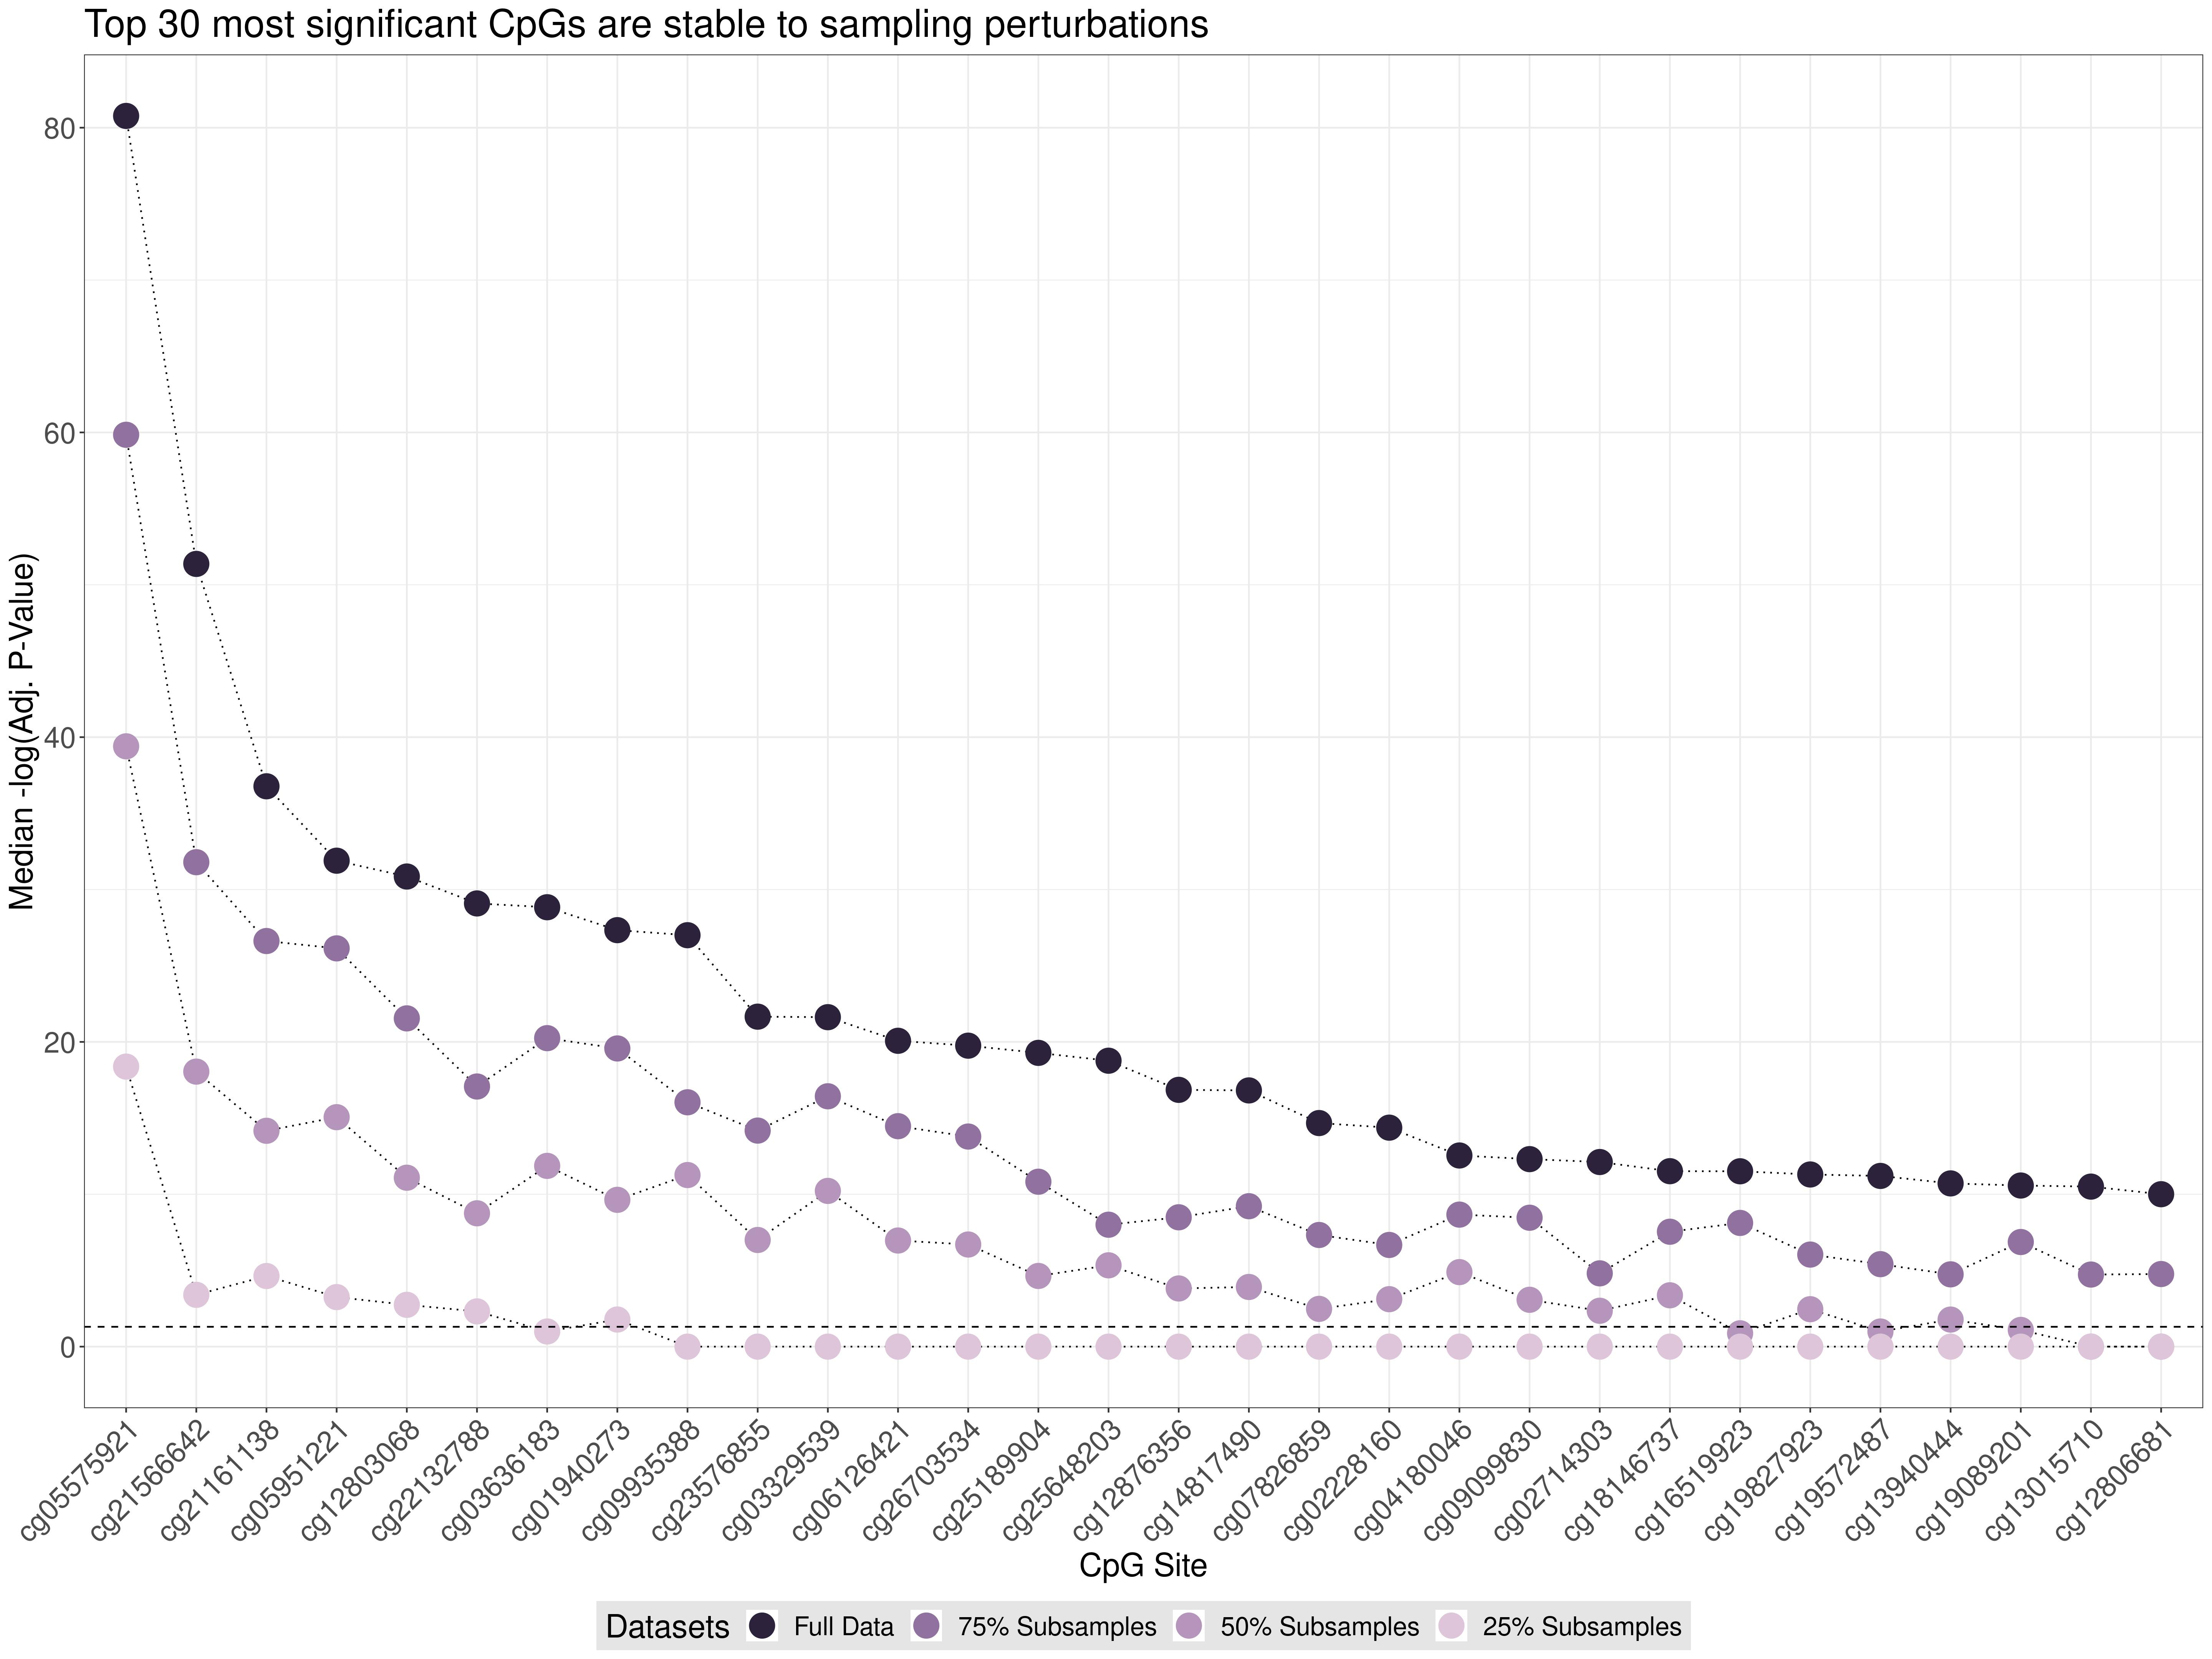
\includegraphics[origin=c,scale=0.22]{cpg_ranks}

\note{
}
\end{frame}

%%%%%%%%%%%%%%%%%%%%%%%%%%%%%%%%%%%%%%%%%%%%%%%%%%%%%%%%%%%%%%%%%%%%%%%%%%%%%%%%

\begin{frame}[c]{Open-source software: \texttt{R/biotmle}!}

\begin{center}
\begin{itemize}
  \itemsep6pt
  \item \texttt{R} package for differential expression or methylation analysis
     based on model-agnostic, efficient estimators of the ATE.
  \item Incorporates machine learning and allows cross-validation.
  \item Statistical inference based on variance \textit{moderation}.
  \item Where can you find it?
    \begin{itemize}
      \itemsep4pt
      \item \url{https://github.com/nhejazi/biotmle}
      \item \url{https://bioconductor.org/packages/biotmle}
    \end{itemize}
\end{itemize}
\end{center}

\note{Use it. File an issue. Help make it better!
}
\end{frame}

%%%%%%%%%%%%%%%%%%%%%%%%%%%%%%%%%%%%%%%%%%%%%%%%%%%%%%%%%%%%%%%%%%%%%%%%%%%%%%%%

\begin{frame}[c]{Review}
\begin{center}
\begin{enumerate}
  \itemsep6pt
  \item Modern computational biology research produces complex, heterogeneous
    data --- innovative statistical inference still tied to simplistic and
    challenging-to-verify modeling assumptions.
  \item \textit{Model misspecification} seriously undermines the scientific
    utility of common, classical statistical modeling approaches.
  \item Non-/semi-parametric inference allows constructing robust estimators
    that easily bring machine learning into the fold.
  \item Variance moderation strengthens hypothesis testing strategies, reducing
    false positives and preserving power under instability.
\end{enumerate}
\end{center}


\note{It's always good to include a summary.}
\end{frame}

%%%%%%%%%%%%%%%%%%%%%%%%%%%%%%%%%%%%%%%%%%%%%%%%%%%%%%%%%%%%%%%%%%%%%%%%%%%%%%%%

% don't want dimming with references
\setbeamercovered{}
\beamerdefaultoverlayspecification{}

\begin{frame}[c,allowframebreaks]{}

\small
\bibliographystyle{apalike}
%\nocite{*}
\bibliography{references}

\end{frame}

%%%%%%%%%%%%%%%%%%%%%%%%%%%%%%%%%%%%%%%%%%%%%%%%%%%%%%%%%%%%%%%%%%%%%%%%%%%%%%%%

\begin{frame}[c]{Thank you}


\includegraphics[scale=0.14]{homepage.png} \url{https://nimahejazi.org}

\vspace{2mm}

\includegraphics[scale=0.11]{github-icon.png}
  \url{https://github.com/nhejazi}

\vspace{2mm}

\includegraphics[scale=0.14]{twitter-icon.png}
  \url{https://twitter.com/nshejazi}

\vspace{2mm}

\includegraphics[scale=0.14]{pdf-icon.png}
  \url{https://doi.org/10.1177/09622802221146313}

\vspace{2mm}

\includegraphics[scale=0.14]{pdf-icon.png}
  \url{https://arxiv.org/abs/1710.05451}

\note{Here's where you can find me, as well as the slides for this talk.}

\end{frame}

\end{document}
